%\documentclass[12pt, oneside]{article}
\documentclass[review]{elsarticle}
\usepackage{lineno,hyperref}
\modulolinenumbers[5]
%\includegraphics
\usepackage[margin=1in]{geometry}
%\geometry{letterpaper}
%\usepackage[parfill]{parskip}
\usepackage{graphicx}
%\usepackage{authblk}
%\usepackage{amssymb}
%\usepackage{cite}
%\usepackage{float}
%\usepackage{fixltx2e}
\usepackage{placeins}
%\usepackage{verbatim}
\usepackage{comment}

\journal{Journal of Nuclear Materials}
\bibliographystyle{elsarticle-num}

\begin{document}
\begin{frontmatter}
\title{Effect of strain and temperature on the threshold displacement energy in body-centered cubic iron}

\author[davisa,berka]{Benjamin Beeler\corref{qwe}}
\cortext[qwe]{Corresponding author}
\ead{bwbeeler@ucdavis.edu}
\author[berka]{Mark Asta}
\author[berkb]{Peter Hosemann}
\author[davisa,davisb]{Niels Gr$\o$nbech-Jensen}
\address[davisa]{Department of Mechanical and Aerospace Engineering, University of California, Davis, CA 95616}
\address[berka]{Department of Materials Science, University of California, Berkeley, CA 94720}
\address[berkb]{Department of Nuclear Engineering, University of California, Berkeley, CA 94720}
\address[davisb]{Department of Mathematics, University of California, Davis, CA 95616}

\begin{abstract}
The threshold displacement energy (TDE) is the minimum amount of kinetic energy required to permanently displace an atom from its lattice site.  The magnitude of the TDE displays significant variance as a function of the crystallographic direction, system temperature and applied strain, among a variety of other factors.  It is critically important to determine an accurate value of the TDE in order to calculate the total number of displacements due to a given irradiation condition, and thus to understand the materials response to irradiation.  In this study, molecular dynamics simulations have been performed to calculate the threshold displacement energy at two separate temperatures and under three separate strain conditions, for ten individual primary knock-on atom (PKA) directions.  It is found that the magnitude of the TDE varies dramatically as a function of PKA direction, and shows significant variance as a function of both strain and temperature.
\end{abstract}
\end{frontmatter}

\linenumbers

\section{Introduction}

Structural materials for nuclear fission and fusion applications experience a dynamic temperature, irradiation and mechanical loading environment.  Understanding materials response to irradiation in this dynamic environment is one of the key issues for the design and operation of nuclear power systems.  Lifetime and operational restrictions are typically influenced by limitations associated with the degradation of structural materials properties under irradiation.  The ability to accurately predict and understand behavior of structural materials under short term and long term irradiation is thus important for designing improved materials for nuclear power applications.  Extensive computational research has been performed in order to better understand radiation damage in widely used structural materials, including ferritic alloys based on body-centered cubic (BCC) iron (Fe) \cite{bacon1993, stoller1996, gao1996, gao1997, becquart1997, stoller1999, malerba2006}.  

Common areas of interest with regards to radiation damage simulations have been general damage behavior \cite{averback1998, phythian1995, bacon1994}, variations in primary knock-on atom (PKA) energy \cite{caturla2000, zinkle1993}, variations in simulation temperature during irradiation \cite{gao1997, phythian1995, soneda1998, bacon2004}, the behavior and effect of extrinsic particles \cite{hayward2010, ackland2004, terentyev2006}, and recently the effect of strain \cite{beeler2015, miyashiro2011, di2013}.  A relatively understudied area of radiation damage is the investigation of the threshold displacement energy.

The threshold displacement energy (TDE) is the minimum amount of kinetic energy required to permanently displace an atom from its lattice site.  This quantity plays a key role in radiation damage theory, where it is implemented within the Kinchin-Pease \cite{kinchinpease} or the NRT \cite{norgett1975} equations, which state that the amount of damage is proportional to the ratio of the amount of deposited energy to an effective TDE.  Therefore, it is critically important to determine an accurate value of the TDE in order to calculate the total number of displacements due to a given irradiation condition, and thus understand the materials response to irradiation.

There is a long, but somewhat limited, history of investigating the TDE in BCC Fe.  Nordlund, \textit{et al.} \cite{nordlund2006} excellently outlined the early history of TDE studies and it will not be repeated here.  Somewhat more recently, Bacon, \textit{et al.} \cite{bacon1993} investigated BCC Fe at 0 K and calculated the TDE as a function of angle with a Finnis-Sinclair potential.  Ackland, \textit{et al.} \cite{ackland1997} performed a similar study at 0 K using a many-body Finnis-Sinclair potential to investigate the effects of dilute Cu on the TDE.  Nordlund \textit{et al.} \cite{nordlund2006} performed an extensive study of 11 separate interatomic potentials to investigate the lower bound of the TDE in BCC Fe at 36 K.  Zolnikov, \textit{et al.} \cite{zolnikov2015} studied the TDE in BCC Fe and V with very high applied tetragonal shear and varying temperature, with an emphasis on plastic deformation.  

The investigation into the effects of applied strain on radiation damage generation in BCC Fe \cite{beeler2015} showed that with certain types of strain, there can be dramatic increases or decreases in the amount of defect accumulation from a given cascade.  This led to a brief investigation into the displacement energy for a single PKA direction in a system with and without strain.  It was shown that applied hydrostatic expansion leads to a decrease in the threshold displacement energy.  A more expansive investigation into the TDE as a function of strain and temperature is thus warranted, and is the focus of this study.

In this paper, molecular dynamics (MD) \cite{abraham1986, allen1987} simulations have been performed to calculate the threshold displacement energy in BCC Fe at 300 K and 500 K, under three separate strain conditions - unstrained, applied tetragonal shear (Bain strain), and applied hydrostatic expansion - for ten individual PKA directions.  The probability of Frenkel pair production is determined as a function of PKA direction, strain and temperature.  Probability curves are averaged to determine average threshold displacement energies.  The minimum amount of kinetic energy required to create a Frenkel pair is also calculated as a function of strain, temperature and PKA direction.

\section{Computational Details}
Molecular dynamics simulations are performed utilizing the LAMMPS \cite{plimpton1995} software package and the Embedded-Atom Method (EAM) \cite{daw1984} interatomic potential developed for BCC Fe by Mendelev \textit{et al.} \cite{mendelev2003}.  To generate probability curves in section 3.1, a BCC supercell containing 16,000 atoms is relaxed for 100 ps at a given temperature in an NPT ensemble.  A strain is applied to the supercell and the strained lattice is allowed to relax for 100 ps in an NVT ensemble.  An atom near the center of the supercell is then given extra kinetic energy, with the velocity directed in varying prescribed directions.  The time step is set to 0.2 fs and the simulation is run for 30000 steps.  We utilize the GJF thermostat \cite{gjf2013, gjf2014} (fix langevin gjf) due to its robust configurational sampling properties.  The damping parameter (analogous to relaxation time) is set to 1 ps.  The number of stable Frenkel pairs is determined after 6 ps via a Wigner-Seitz cell based algorithm \cite{hayward2010}.  Thus, this analysis does not take into account long-time thermal diffusion.  PKA energies are varied over a range of approximately 100 eV, in steps of 2.5-10 eV, to properly sample the relevant energy range.  The PKA directions analyzed are ten random directions that adequately sample the BCC crystal cell \cite{beeler2015}.  The description of each of these ten directions is outlined in Appendix A.  For each strain state and PKA direction, 64-100 independent simulations are performed, each with a unique distribution of initial velocities.  To determine the minimum value of the threshold displacement energy in section 3.2, a BCC supercell containing 2,000 atoms is relaxed for 100 ps at a given temperature in an NPT ensemble.  A strain is applied to the supercell and the strained lattice is allowed to relax for 60 ps in an NVT ensemble.  An atom near the center of the supercell is then given extra kinetic energy, with the velocity directed in varying prescribed directions.  The time step is set to 0.2 fs and the simulation is run for 30000 steps.  The number of stable Frenkel pairs is determined after 6 ps via a Wigner-Seitz cell based algorithm \cite{hayward2010}.  PKA energies are varied in steps of 2 eV, to properly sample the relevant energy range.  The same set of PKA directions is utilized, as outlined in Appendix A.  Further details regarding the specifications of the applied strain have been outlined previously \cite{beeler2015}.

How the TDE is defined is not exactly straight-forward, in that it can, and should, vary depending on the type of investigation one intends to perform.  This was outlined by Nordlund \cite{nordlund2006}, where several different types of TDE were explained and calculated.  In the previous literature, the primary type of TDE reported is the E$^{l}_{d}$, or the lower bound of the displacement energy, where there exists a non-zero probability of creating a defect (a defect is sometimes produced) \cite{malerba2002}.  Typically, the direct experimental measurements of the TDE measure the lowest electron energy where a defect signal can be detected, for example by changes in resistivity.  This is analagous to the E$^{l}_{d}$.  For comparison to experiment, adjustments for beam spreading should be included \cite{nordlund2006}.  For implementation into the Kinchin-Pease or NRT equations, an average value for the TDE needs to be utilized.  This average value is obtained from generating probability curves (probability of generating a Frenkel pair as a function of PKA energy) for respective PKA directions.  These probability curves can then be angularly averaged to create an angle-integrated displacement probability curve \cite{nordlund2006}.  The energy at which this averaged probability curve crosses the probability 0.5 is determined to be the average TDE (E$^{avg}_{d}$).  Both the E$^{avg}_{d}$ and the E$^{l}_{d}$ are calculated in this work.


\section{Results}
\subsection{Average Threshold Displacement Energy}
In this section, E$^{avg}_{d}$ is determined through a variety of simulations.  This is the proper value of the TDE for implementation into the Kinchin-Pease or NRT equations.  This value takes into account not only displacement of atoms, but allows for subsequent recombination.  The results below in Figure 1 outline each of the ten random directions investigated, and illustrate the probability of Frenkel pair production as a function of the PKA energy.  Each direction has two associated graphs.  The first graph includes data points and fourth-order polynomial fits to these data points.  The second associated graph only includes the polynomial fits, to better illustrate the general trends the data exhibit.  In all graphs, the red square data points and the red dashed line denote a system without external applied strain.  In all graphs, the blue diamond data points and the blue solid line denote a system with 2$\%$ hydrostatic expansion.  Results for applied 5$\%$ Bain strain are excluded from these graphs for the sake of clarity.

\begin{figure}[hp]
   \centering
   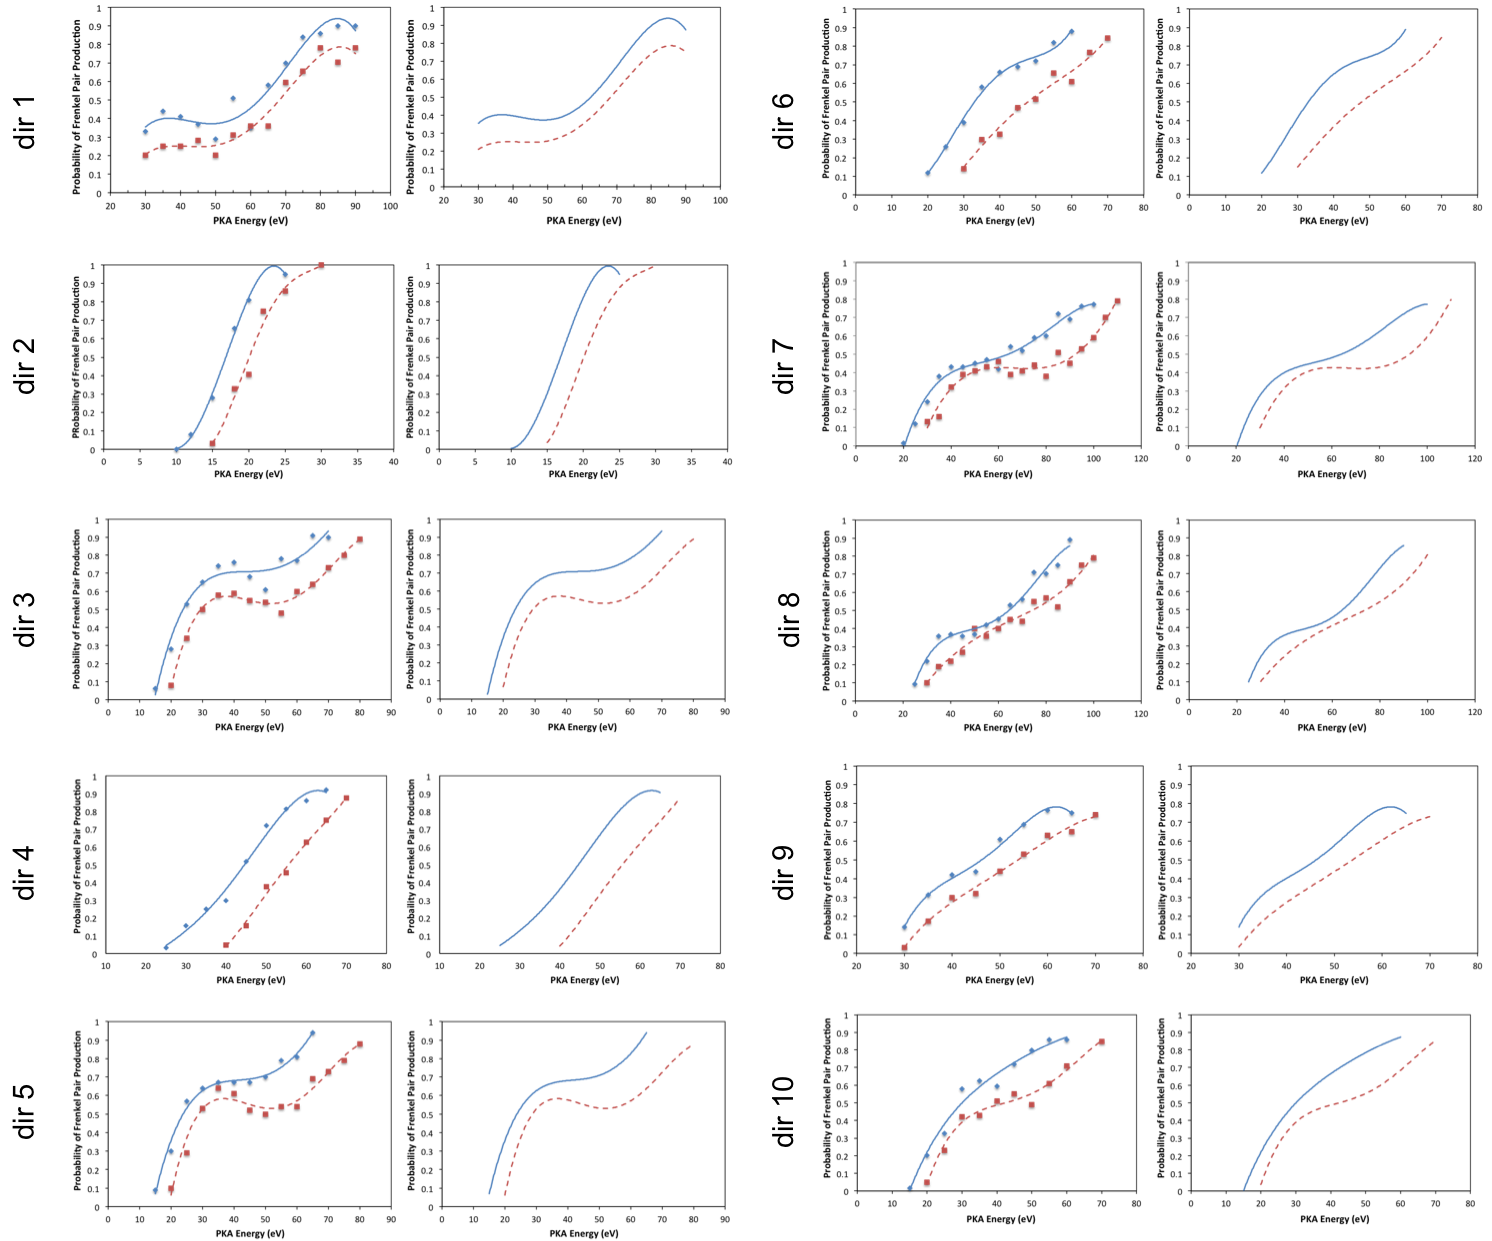
\includegraphics[width=\textwidth]{fig_all.png} % requires the graphicx package
   \caption{Probability of Frenkel pair production as a function of PKA energy at 300 K for ten random PKA directions.  The red square data points and the red dashed line denote a system without external applied strain.  The blue diamond data points and the blue solid line denote a system with 2$\%$ hydrostatic expansion.  Each direction has two associated graphs: the first graph includes data points and fourth-order polynomial fits to these data points, the second associated graph only includes the polynomial fits.  The directions are labeled from \textit{dir 1} to \textit{dir 10}.}
   \label{fig:example}
\end{figure}

There are numerous interesting details from the these twenty graphs.  The first is the general behavior of the probability of Frenkel pair production as a function of PKA energy.  Since TDE is thought of as a threshold, it would be expected that these graphs would be near step-functions, with some scatter as a result of thermal fluctuations.  However, there are large ranges in energy for nearly all investigated directions where the probability to create a Frenkel pair is non-zero and non-negligible.  This suggests it would be more accurate to utilize the entire probability versus PKA energy curve to realize the actual dpa under irradiation.  Also, there often exists a plateauing of the probability curve.  This can be understood as due to excess heat leading to increased recombination.  As the PKA energy increases, it finally becomes large enough to overcome this increase in recombination, leading to an increase in the probability of defect formation.  The second key feature of the graphs is the relative probabilities for a given PKA energy with and without applied strain.  Nearly universally, for a given PKA energy, the probability of creating a Frenkel pair is greater for a system with applied 2$\%$ hydrostatic expansion.  There is some uncertainty within the data, leading to scatter, but analyzing the polynomial fits clearly shows the general trends of the data: that it is more likely to create a Frenkel pair from a PKA with a given energy in a system with 2$\%$ applied hydrostatic strain compared to a system with no applied external strain.  This shows that the TDE is in fact affected by applied strain.  Thirdly, it is clear that the general behavior of the probability versus energy curves varies greatly as a function of PKA direction.  This emphasizes the strong crystallographic dependence of the TDE and the need for investigation over a variety of PKA directions.

Using this data, we want to analyze the actual value of the TDE for each direction.  The point at which the probability curve becomes greater than or equal to 0.5 is taken as the value of the TDE for that specific PKA direction.  Thus, the TDE is the energy when it becomes probable that a defect is created.  A summary of the TDE across all ten directions is shown in Figure 2.  This data is for systems at 300 K and 500 K, for all three investigated strain systems.  

\begin{figure}[hp]
   \centering
   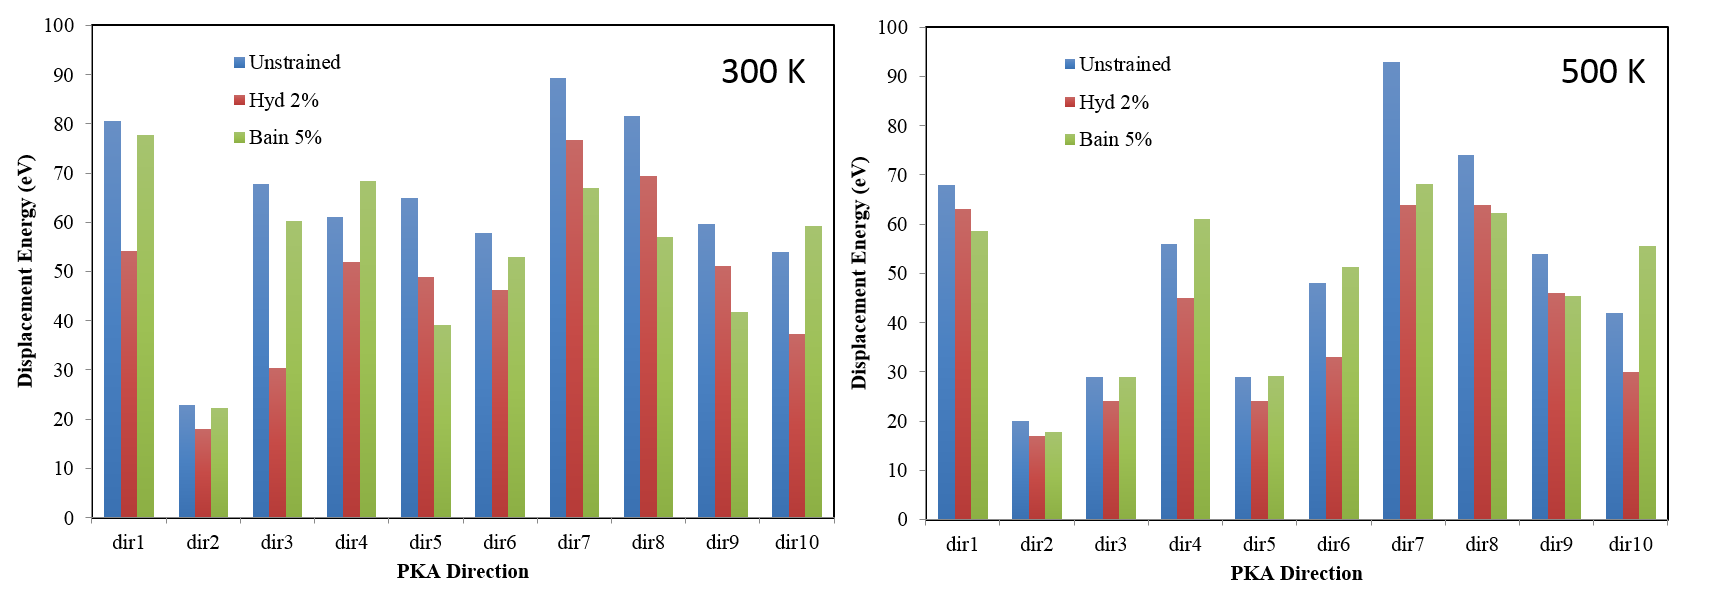
\includegraphics[width=\textwidth]{bar_charts.png} % requires the graphicx package
   \caption{The threshold displacement energy as a function of direction at 300 K and 500 K.  The blue bars denote a system without external applied strain.  The red bars denote a system with 2$\%$ hydrostatic expansion. The green bars denote a system with 5$\%$ Bain strain.}
   \label{fig:example}
\end{figure}

The data from Figure 2 is tabulated in Table 1 and Table 2.  At 300 K, across all directions, there is a decrease in the TDE for applied hydrostatic strain, from a minimum difference of 3 eV, to a maximum of 29 eV.  For applied Bain strain, there is a decrease in the TDE for five directions, with a maximum decrease of 25 eV.  For two directions there is no change in the TDE and for three directions there is an increase in the TDE.  This again highlights the importance of conducting investigations over a variety of PKA directions.  At 500 K, across all directions, there is also a decrease in the TDE for applied hydrostatic strain, from a minimum difference of 5 eV, to a maximum of 38 eV.  For applied Bain strain, there is a decrease in the TDE for eight directions, with a maximum decrease of 26 eV.  For two directions there is an increase in the TDE.  

\begin{table}[htbp]
\caption{The threshold displacement energy as a function of direction at 300 K for three strain conditions.  Energies given in eV.}
\begin{center}
\begin{tabular}{|c|c|c|c|}
	\hline
	& Unstrained & Hydrostatic 2$\%$ & Bain 5$\%$ \\
	 \hline
	 dir 1 & 68 & 63 & 59 \\
	 dir 2 & 20 & 17 & 18 \\
	 dir 3 & 29 & 24 & 29 \\
	 dir 4 & 56 & 45 & 61 \\
	 dir 5 & 29 & 24 & 29 \\
	 dir 6 & 48 & 33 & 51 \\
	 dir 7 & 93 & 64 & 68 \\
	 dir 8 & 74 & 64 & 62 \\
	 dir 9 & 54 & 46 & 46 \\
	 dir 10 & 42 & 30 & 56 \\
	 \hline
\end{tabular}
\end{center}
\label{default}
\end{table}%

\begin{table}[htbp]
\caption{The threshold displacement energy as a function of direction at 500 K for three strain conditions.  Energies given in eV.}
\begin{center}
\begin{tabular}{|c|c|c|c|}
	\hline
	& Unstrained & Hydrostatic 2$\%$ & Bain 5$\%$ \\
	 \hline
	 dir 1 & 81 & 54 & 78 \\
	 dir 2 & 23 & 18 & 22 \\
	 dir 3 & 68 & 30 & 60 \\
	 dir 4 & 61 & 52 & 68 \\
	 dir 5 & 65 & 49 & 39 \\
	 dir 6 & 58 & 46 & 53 \\
	 dir 7 & 89 & 77 & 67 \\
	 dir 8 & 82 & 69 & 57 \\
	 dir 9 & 60 & 51 & 42 \\
	 dir 10 & 54 & 37 & 59 \\
	 \hline
\end{tabular}
\end{center}
\label{default}
\end{table}%

\FloatBarrier

The probability curves displayed in Figure 1 are averaged, creating a single angle-integrated probability curve for each of the three strain conditions.  These three probability curves are displayed in Figure 3, for the system at 300 K and 500 K.  The value of E$^{avg}_{d}$ is calculated from the point where the curve crosses 0.5 probability.  The values of E$^{avg}_{d}$ at 300 K for the unstrained, hydrostatic 2$\%$ and Bain $5\%$ are 49 eV, 36 eV and 47 eV, respectively.  The values of E$^{avg}_{d}$ at 500 K for the unstrained, hydrostatic 2$\%$ and Bain $5\%$ are 58 eV, 45 eV and 53 eV, respectively.  It should be noted that the standard value for the TDE in iron is usually taken as 40 eV \cite{was2007}.  This value is for a system at 0 K, and thus thermal fluctuations at 300 K and 500 K are dictating an increase in the TDE to a value of 49 eV and 59 eV, respectively.

\begin{figure}[hp]
   \centering
   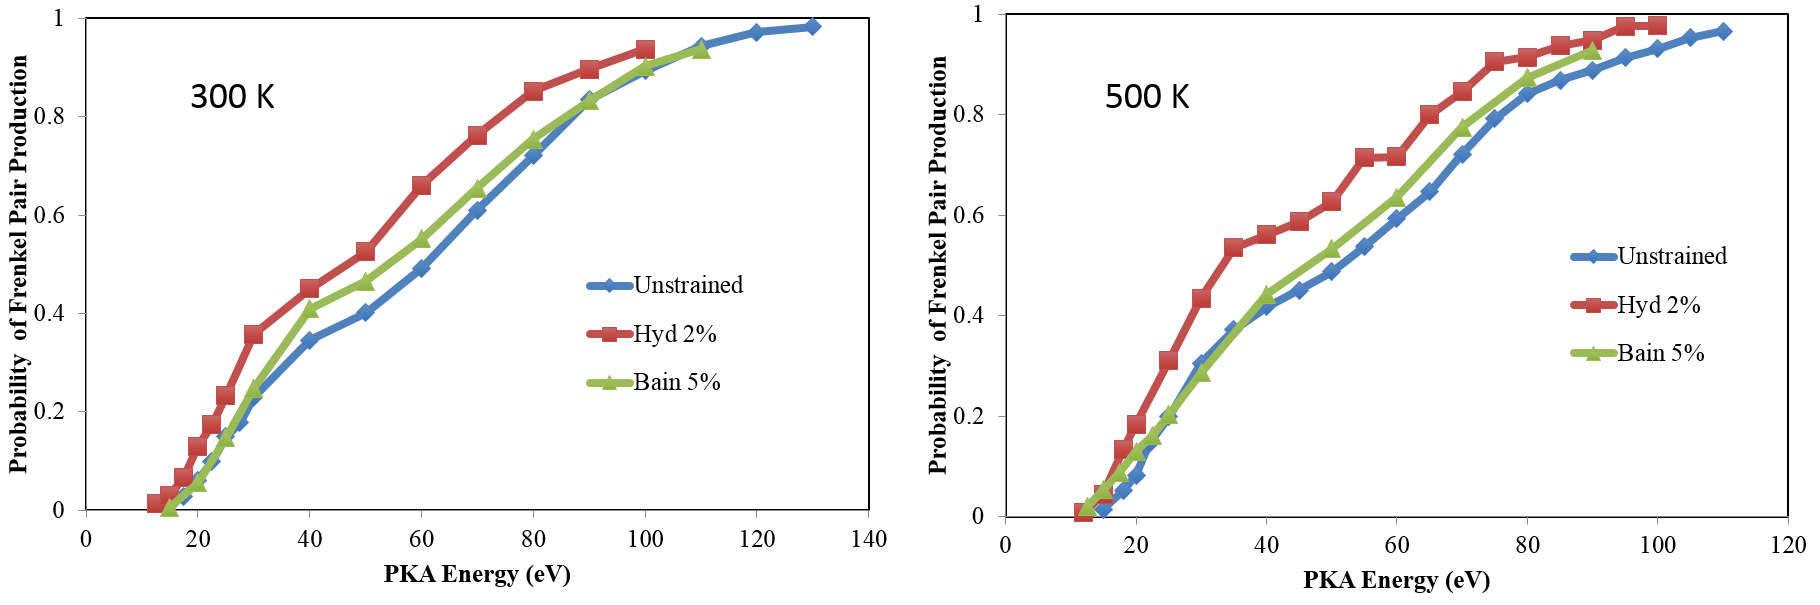
\includegraphics[width=\textwidth]{pp_curves.png} % requires the graphicx package
   \caption{The angle-integrated probability curves at 300 K and 500 K for three strain conditions.  The blue diamond data points denote a system without external applied strain.  The red square data points denote a system with 2$\%$ hydrostatic expansion. The green triangle data points denote a system with 5$\%$ Bain strain.}
   \label{fig:example}
\end{figure}

Figure 3 shows that with applied hydrostatic expansion, there is a marked shift left of the probability curve for both temperatures.  Thus, for a given PKA energy, it is more likely to create a Frenkel pair in a system under 2$\%$ hydrostatic expansion, than in an unstrained system.  Thus, one would expect a higher number of defects created under higher energy PKAs.  This is consistent with previous work \cite{beeler2015}.  This also illustrates that there is an overall decrease of 13 eV in the TDE at 300 K and 500 K that would be used as an input into the Kinchin-Pease or NRT radiation damage models.  For applied Bain strain at 300 K, there exists a very minor shift left of the probability curve, yielding minimal changes to the average radiation damage response of the material.  This is also consistent with previous work \cite{beeler2015}.  However, the shift is more substantial for simulations at 500 K.  Application of 5$\%$ Bain strain at 500 K yields a decrease in the E$^{avg}_{d}$ of 5 eV.

\FloatBarrier

A comparison of the above results for temperatures at 300K and 500 K is tabulated in Table 3.  For all strain conditions, an increase in temperature yields an increase in the E$^{avg}_{d}$.  For both temperatures, the unstrained system exhibits the highest displacement energy and the system under 2$\%$ hydrostatic expansion exhibits the lowest displacement energy.  The largest variance in the TDE with respect to strain has a magnitude of 13.5 eV.  The largest variance in the TDE with respect to temperature is 9.4 eV.  In the Kinchin-Pease and NRT equations, the number of displacements is inversely proportional to the TDE.  If we take as an example the unstrained system of BCC Fe, using the TDE value at 300 K yields approximately 18$\%$ more displacements than if the value of TDE at 500 K is utilized and 18$\%$ fewer displacements than if the typical value for BCC Fe of 40 eV is utilized.  This underlines the importance of the proper implementation of the appropriate E$^{avg}_{d}$ for a particular system.  

\begin{table}[htbp]
\caption{The average threshold displacement energy in BCC Fe at three strain conditions and two temperatures.  Energies given in eV.}
\begin{center}
\begin{tabular}{|c|c|c|}
	\hline
	& 300 K & 500 K \\
	 \hline
	 Unstrained & 49 & 58.1 \\
	 Hyd 2$\%$ & 35.5 & 44.9 \\
	 Bain 5$\%$ & 46.8 & 52.8 \\
	 \hline
\end{tabular}
\end{center}
\label{default}
\end{table}

\FloatBarrier
\subsection{Lower Bound of the Threshold Displacement Energy}

Typically, the direct experimental measurements of the TDE measure the lowest electron energy where a defect signal can be detected, for example by changes in resistivity.  This is analogous to the lower bound of the threshold displacement energy, E$^{l}_{d}$.  The E$^{l}_{d}$ is the lowest possible value of kinetic energy such that a Frenkel pair can be created.  In this work, the minimum probability to meet the criterion for defect production is 0.01.   The results for the E$^{l}_{d}$ as a function of PKA direction and temperature are displayed in Figure 4, for all three strain conditions.  

From Figure 4, it is found that the magnitude of E$^{l}_{d}$ varies from 10 eV at the minimum to 26 eV at the maximum across all PKA directions and temperatures.  There is a strong dependence of the E$^{l}_{d}$ as a function of crystallographic direction.  These results are numerically averaged to determine the average E$^{l}_{d}$ for each strain condition and temperature.  These results are tabulated in Table 4.

\begin{figure}[hp]
   \centering
   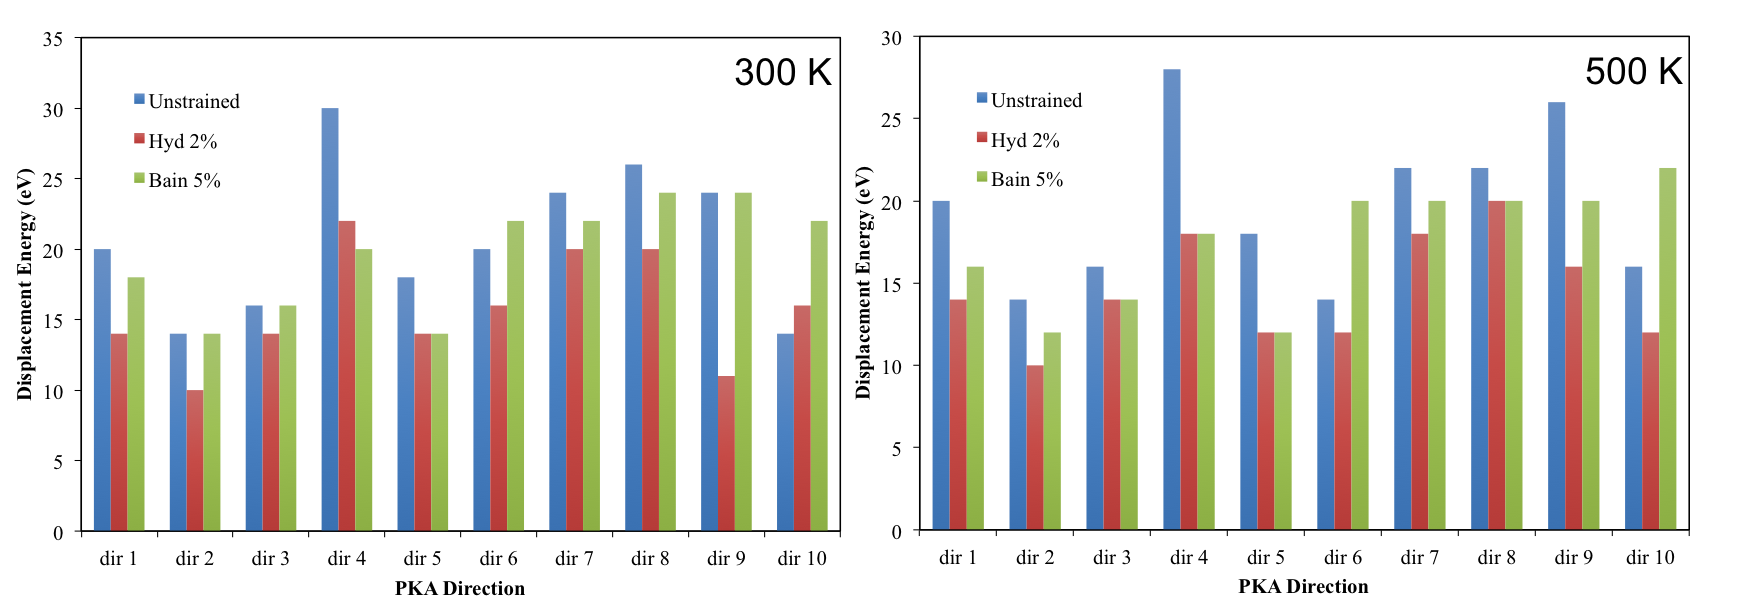
\includegraphics[width=\textwidth]{bar_charts2.png} % requires the graphicx package
   \caption{The lower bound threshold displacement energy as a function of direction at 300 K and 500 K.  The blue bars denote a system without external applied strain.  The red bars denote a system with 2$\%$ hydrostatic expansion. The green bars denote a system with 5$\%$ Bain strain.}
   \label{fig:example}
\end{figure}


\FloatBarrier

\begin{table}[htbp]
\caption{The lower bound of the threshold displacement energy in BCC Fe at three strain conditions and two temperatures.  Energies given in eV.  Plus/minus is the standard error of the mean.}
\begin{center}
\begin{tabular}{|c|c|c|}
	\hline
	& 300 K & 500 K \\
	 \hline
	 Unstrained & 20.6 $\pm 1.69$ & 19.6 $\pm 1.54$ \\
	 Hyd 2$\% $  & 15.7 $\pm 1.25$ & 14.6 $\pm 1.03$ \\
	 Bain 5$\%$  & 19.6 $\pm 1.22$ & 17.4 $\pm 1.16$ \\
	 \hline
\end{tabular}
\end{center}
\label{default}
\end{table}

For both temperatures, the unstrained system exhibits the highest displacement energy and the system under 2$\%$ hydrostatic expansion exhibits the lowest displacement energy, consistent with the results in Table 3 for E$^{avg}_{d}$.  However, for all strain conditions, the E$^{l}_{d}$ at 300 K is higher than at 500 K.  This is in direct contrast to the results in Table 3.  Thus, the E$^{l}_{d}$ and the E$^{avg}_{d}$ exhibit opposite behaviors as a function of temperature from 300 K to 500 K.  This can be explained by the nature of these two different definitions of the TDE.  For E$^{avg}_{d}$, higher energy PKAs are utilized, inducing mini-cascades.  Additional thermal fluctuations can allow for increased recombination as the thermal spike anneals.  For E$^{l}_{d}$, increased thermal fluctuations can act to rapidly diffuse a created interstitial away from the resultant vacancy, creating a stable Frenkel pair.  Thus, an increase in temperature yields an increase in the probability for a set of PKAs to create a $\it{single}$ Frenkel pair (E$^{l}_{d}$), while yielding a decrease in the $\it{overall}$ probability of creating a Frenkel pair (E$^{avg}_{d}$).

The traditional value used for the E$^{l}_{d}$ in BCC Fe is 20 eV \cite{was2007}, and the results at 300 K and 500 K for the unstrained system are in line with this traditional value.  The maximum variance in the E$^{l}_{d}$ as a function of strain is 5 eV.  The maximum variance in the E$^{l}_{d}$ as a function of temperature is 2.2 eV.  

\section{Conclusions}
In this study, molecular dynamics simulations were performed on pure BCC Fe to investigate the effects of applied strain and temperature on the threshold displacement energy.  Two separate values for the threshold displacement energy are calculated: E$^{avg}_{d}$ and E$^{l}_{d}$.  Each threshold displacement energy is determined as a function of ten PKA directions, three strain conditions, and two temperatures.  It was determined that for E$^{avg}_{d}$, application of 2$\%$ hydrostatic strain results in a decrease of 13.2-13.5 eV and application of 5$\%$ Bain strain results in a decrease of 2.2-5.3 eV.  For E$^{avg}_{d}$, an increase in the temperature of the system from 300 K to 500 K can result in an increase of 6-9.4 eV.  For E$^{l}_{d}$, application of 2$\%$ hydrostatic strain results in a decrease of 4.9-5 eV and application of 5$\%$ Bain strain results in a decrease of 1-2.2 eV.  For E$^{l}_{d}$, an increase in the temperature of the system from 300 K to 500 K can result in a decrease of 1-2.2 eV.  This study clearly shows the importance of accounting for changes in strain environment and system temperature regarding the threshold displacement energy and the resulting radiation damage behavior.  

\section{Acknowledgement}
This work was supported by the US Department of Energy, project $\#$DE-NE0000536000.

\FloatBarrier

\appendix
\section{Set of random directions}

The set of directions are chosen at random from a range of $\theta$ and $\phi$ values based on the body-centered cubic crystal structure and illustrated in Figure A.5.  The specific $\theta$ and $\phi$ values are provided in Table A.5, along with the corresponding \textit{h}, \textit{k}, \textit{l} values.  These \textit{h}, \textit{k}, \textit{l} values are normalized such that \textit{h} is equal to 1.  It was found that this set of directions adequately samples the BCC crystal structure.

\begin{figure}[hp]
   \centering
   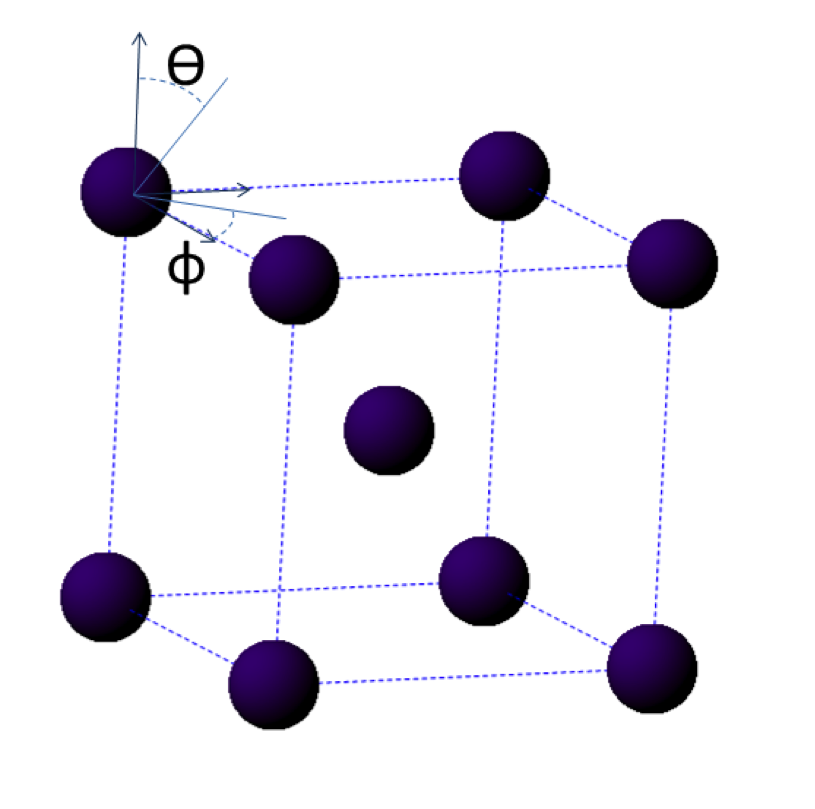
\includegraphics[width=0.5\textwidth]{figure1.png} % requires the graphicx package
   \caption{Random directions were selected for primary knock-on atoms to sample the complete set of directions within a BCC crystal system.  The angle theta ($\theta$) was allowed to vary from 0 to $\pi$/2.  The angle phi ($\phi$) was allowed to vary from 0 to $\pi$/4.}
   \label{fig:example}
\end{figure}

\begin{table}[htbp]
\caption[c]{The set of ten random directions utilized in all simulations.  Values of $\theta$ and $\phi$ are given in degrees.  Values of \textit{h}, \textit{k}, \textit{l} are normalized such that \textit{h} is equal to 1.}
\begin{center}
\begin{tabular}{|c|c|c|c|c|c|}
	\hline
	& $\theta$ & $\phi$ & h & k & l \\
	 \hline
	 dir 1 & 27 & 24 & 1 & 2.25 & 4.83 \\
	 dir 2 & 17 & 5 & 1 & 11.43 & 37.53 \\
	 dir 3 & 24 & 15 & 1 & 3.73 & 8.68 \\
	 dir 4 & 31 & 11 & 1 & 5.14 & 8.72 \\
	 dir 5 & 24 & 14 & 1 & 4.01 & 9.28 \\
	 dir 6 & 86 & 26 & 1 & 2.05 & 0.16 \\
	 dir 7 & 37 & 38 & 1 & 1.28 & 2.16 \\
	 dir 8 & 35 & 44 & 1 & 1.04 & 2.06 \\
	 dir 9 & 85 & 45 & 1 & 1 & 0.12 \\
	 dir 10 & 65 & 4 & 1 & 14.30 & 6.68 \\
	 \hline
\end{tabular}
\end{center}
\label{default}
\end{table}
 
\FloatBarrier

\bibliography{bibliography_ben}


\end{document}  
